\section{Graphs and Properties of Logarithmic Functions}

In this section, you will:
\begin{enumerate}
    \item examine properties of logarithmic functions
    \item examine graphs of logarithmic functions
    \item examine the relationship between graphs of exponential and logarithmic functions
\end{enumerate}


Recall that the exponential function $f(x) = 2^x$ produces this table of values
\[
    \begin{array}{c|ccccccc}
        x    & -3  & -2  & -1  & 0 & 1 & 2 & 3 \\
        \hline
        f(x) & 1/8 & 1/4 & 1/2 & 1 & 2 & 4 & 8 \\
    \end{array}
\]
Since the logarithmic function is an inverse of the exponential, $g(x) = \log_2(x)$ produces the table of values
\[
    \begin{array}{c|ccccccc}
        x    & 1/8 & 1/4 & 1/2 & 1 & 2 & 4 & 8 \\
        \hline
        g(x) & -3  & -2  & -1  & 0 & 1 & 2 & 3 \\
    \end{array}
\]

In this second table, notice that:
\begin{itemize}
    \item As the input increases, the output increases.
    \item As input increases, the output increases more slowly.
    \item Since the exponential function only outputs positive values, the logarithm can only accept positive values as inputs, so the domain of the log function is $(0, \infty)$.
    \item Since the exponential function can accept all real numbers as inputs, the logarithm can have any real number as output, so the range is all real numbers or $(-\infty, \infty)$.
\end{itemize}

Plotting the graph of $g(x) = \log_2(x)$ from the points in the table, notice that as the input values for x approach zero, the output of the function grows very large in the negative direction, indicating a vertical asymptote at $x = 0$.

In symbolic notation we write
\[
    \text{as } x \to 0^+, f(x) \to -\infty
\]
and
\[
    \text{as } x \to \infty, f(x) \to \infty
\]
\begin{center}
    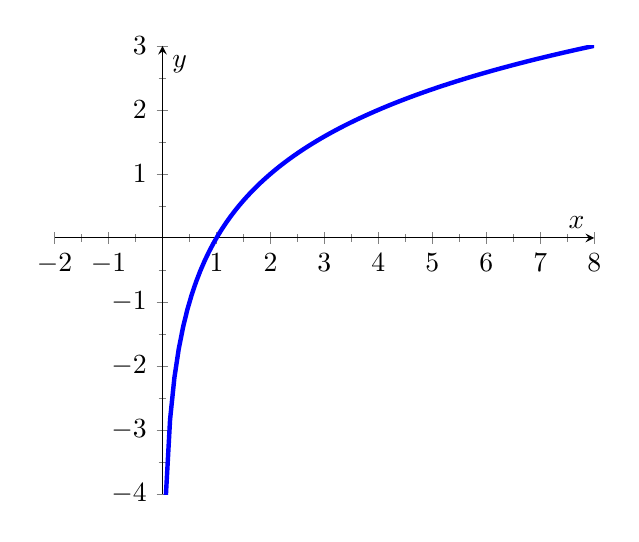
\begin{tikzpicture}
        \begin{axis}[
                axis lines=middle,
                xlabel={$x$},
                ylabel={$y$},
                % xlabel style={at={(axis description cs:1,0)}, anchor=west},
                % ylabel style={at={(axis description cs:0,1)}, anchor=south},
                xtick={-2,-1,...,8},
                ytick={-4,-3,...,3},
                xmin=-2, xmax=8,
                ymin=-4, ymax=3,
                % grid=both,
                % grid style={line width=.1pt, draw=gray!10},
                % major grid style={line width=.2pt, draw=gray!50},
                minor tick num=1, % Subdivision between major ticks
                samples=100,
                domain=0.06:8, % log is not defined for x=0
            ]

            % Plot the function log_2(x)
            \addplot[blue, ultra thick] {log2(x)};
        \end{axis}
    \end{tikzpicture}
\end{center}

Graphically, in the function $g(x) = \log_b(x)$, $b > 1$, we observe the following properties:

\begin{center}
    \begin{tikzpicture}[scale=1]
        \draw[->] (-2,0) -- (5,0) node[right] {$x$};
        \draw[->] (0,-3) -- (0,3) node[above] {$y$};

        \draw[domain=0.1:4.5,smooth,variable=\x,blue, ultra thick] plot ({\x},{log2(\x)});
        % \draw[dotted] (1,-3) -- (1,3);
        \node[] at (2,3) {$y = \log_b(x)$};
        \node[] at (2,2.25) {$b > 1$};

        \node[below right] at (1,0) {(1,0)};
        \node[circle,fill,inner sep=1.5pt] at (1,0) {};

        \node[below right] at (2,1) {$(b,1)$};
        \node[circle,fill,inner sep=1.5pt] at (2,1) {};
    \end{tikzpicture}
\end{center}

\begin{itemize}
    \item The graph has a horizontal intercept at (1, 0).
    \item The line $x = 0$ (the y-axis) is a vertical asymptote; as $x \rightarrow 0^+$, $y \rightarrow -\infty$.
    \item The graph is increasing if $b > 1$.
    \item The domain of the function is $x > 0$, or $(0, \infty)$.
    \item The range of the function is all real numbers, or $(-\infty, \infty)$.
\end{itemize}

However if the base $b$ is less than 1, $0 < b < 1$, then the graph appears as below.

\begin{center}
    \begin{tikzpicture}[scale=1]
        \draw[->] (-2,0) -- (5,0) node[right] {$x$};
        \draw[->] (0,-3) -- (0,3) node[above] {$y$};

        \draw[domain=0.1:4.5,smooth,variable=\x,blue, ultra thick] plot ({\x},{-log2(\x)});
        % \draw[dotted] (1,-3) -- (1,3);
        \node[fill=white] at (3,2.5) {$y = \log_b(x)$};
        \node[fill=white] at (3,2) {$0 < b < 1$};

        \node[below left] at (1,0) {(1,0)};
        \node[circle,fill,inner sep=1.5pt] at (1,0) {};

        \node[above right] at (0.5,1) {$(b,1)$};
        \node[circle,fill,inner sep=1.5pt] at (0.5,1) {};
    \end{tikzpicture}
\end{center}

\begin{itemize}
    \item The graph has a horizontal intercept at (1, 0).
    \item The line $x = 0$ (the y-axis) is a vertical asymptote; as $x \rightarrow 0^+$, $y \rightarrow -\infty$.
    \item The graph is decreasing if $0 < b < 1$.
    \item The domain of the function is $x > 0$, or $(0, \infty)$.
    \item The range of the function is all real numbers, or $(-\infty, \infty)$.
\end{itemize}

When graphing a logarithmic function, it can be helpful to remember that the graph will pass through the points $(1, 0)$ and $(b, 1)$.

Finally, we compare the graphs of \( y = b^x \) and \( y = \log_b(x) \), shown below on the same axes.

Because the functions are inverse functions of each other, for every specific ordered pair $(h, k)$ on the graph of $y = bx$, we find the point $(k, h)$ with the coordinates reversed on the graph of $y = \log_b (x)$.

In other words, if the point with $x = h$ and $y = k$ is on the graph of $y = bx$, then the point with $x = k$ and $y = h$ lies on the graph of $y = \log_b (x)$.

The domain of $y = bx$ is the range of $y = \log_b (x)$. The range of $y = bx$ is the domain of $y = \log_b (x)$.

For this reason, the graphs appear as reflections, or mirror images, of each other across the diagonal line $y = x$. This is because the inputs and outputs are swapped for a function and its inverse.


\begin{center}
    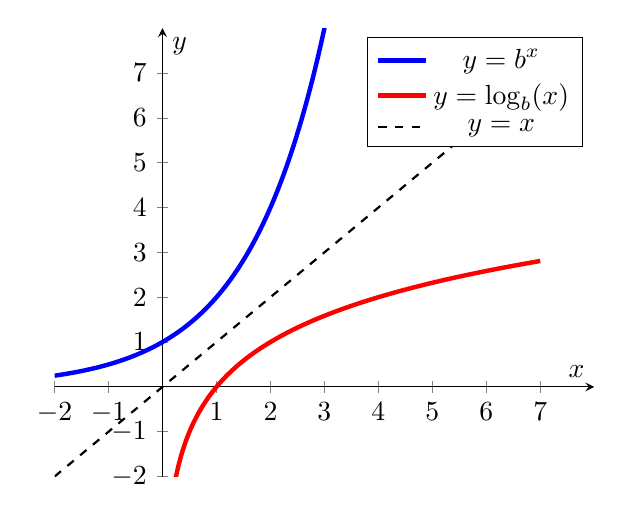
\begin{tikzpicture}
        \begin{axis}[
                axis lines=middle,
                xlabel=\( x \),
                ylabel=\( y \),
                ymin=-2, ymax=8,
                xmin=-2, xmax=8,
                domain=0:3,
                samples=100,
                xtick={-2,...,7},
                ytick={-2,...,7}
            ]
            % Add the exponential function
            \addplot[domain=-2:4.5,smooth,blue, ultra thick] {exp(ln(2)*x)};
            \addlegendentry{\( y = b^x \)}

            % Add the logarithmic function
            \addplot[domain=.01:7,smooth,red, ultra thick] {ln(x)/ln(2)};
            \addlegendentry{\( y = \log_b(x) \)}

            % Add the line y = x
            \addplot[domain=-2:7,black, dashed, thick] {x};
            \addlegendentry{\( y = x \)}

        \end{axis}
    \end{tikzpicture}
\end{center}

